\documentclass{standalone}
\usepackage{tikz}
\usetikzlibrary{patterns, positioning}

\begin{document}
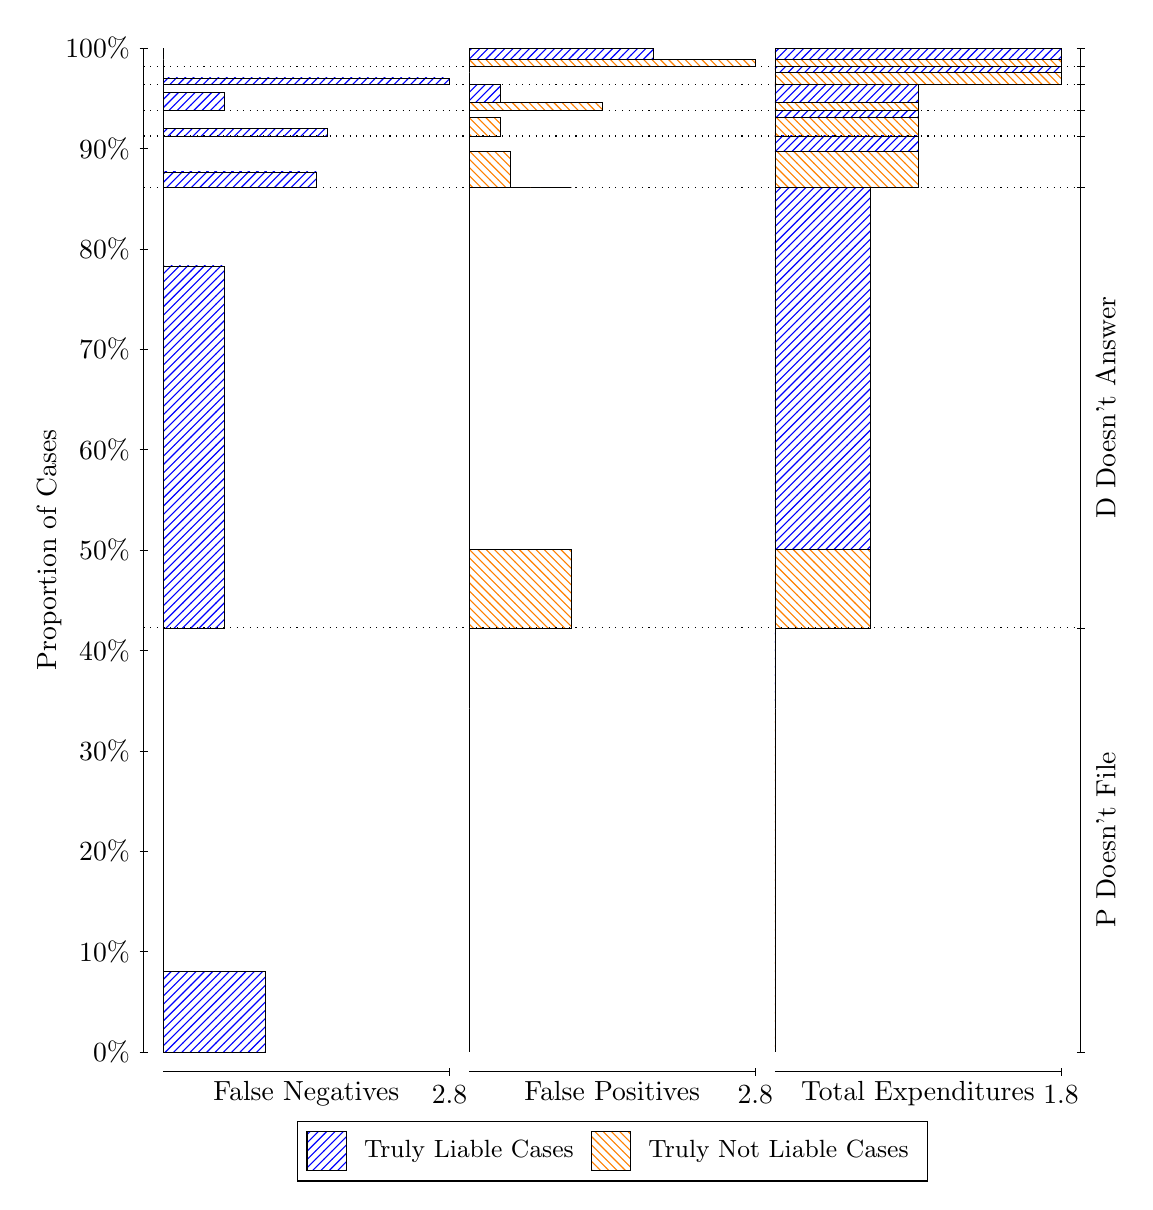
\begin{tikzpicture}
\draw[black, very thin] (1.5,1.75) -- (1.5,14.5);
\node[rotate=90, anchor=center] at (0.3, 8.125) {Proportion of Cases};
\draw[black, very thin] (1.45,1.75) -- (1.55,1.75);
\node[anchor=east] at (1.45, 1.75) {0\%};
\draw[black, very thin] (1.45,3.025) -- (1.55,3.025);
\node[anchor=east] at (1.45, 3.025) {10\%};
\draw[black, very thin] (1.45,4.3) -- (1.55,4.3);
\node[anchor=east] at (1.45, 4.3) {20\%};
\draw[black, very thin] (1.45,5.575) -- (1.55,5.575);
\node[anchor=east] at (1.45, 5.575) {30\%};
\draw[black, very thin] (1.45,6.85) -- (1.55,6.85);
\node[anchor=east] at (1.45, 6.85) {40\%};
\draw[black, very thin] (1.45,8.125) -- (1.55,8.125);
\node[anchor=east] at (1.45, 8.125) {50\%};
\draw[black, very thin] (1.45,9.4) -- (1.55,9.4);
\node[anchor=east] at (1.45, 9.4) {60\%};
\draw[black, very thin] (1.45,10.675) -- (1.55,10.675);
\node[anchor=east] at (1.45, 10.675) {70\%};
\draw[black, very thin] (1.45,11.95) -- (1.55,11.95);
\node[anchor=east] at (1.45, 11.95) {80\%};
\draw[black, very thin] (1.45,13.225) -- (1.55,13.225);
\node[anchor=east] at (1.45, 13.225) {90\%};
\draw[black, very thin] (1.45,14.5) -- (1.55,14.5);
\node[anchor=east] at (1.45, 14.5) {100\%};

\draw[black, very thin] (13.4,1.75) -- (13.4,14.5);
\draw[black, very thin] (13.35,1.75) -- (13.45,1.75);
\node[anchor=west] at (13.35, 1.75) {};
\draw[black, very thin] (13.35,7.1369) -- (13.45,7.1369);
\node[anchor=west] at (13.35, 7.1369) {};
\draw[black, very thin] (13.35,12.73) -- (13.45,12.73);
\node[anchor=west] at (13.35, 12.73) {};
\draw[black, very thin] (13.35,13.383) -- (13.45,13.383);
\node[anchor=west] at (13.35, 13.383) {};
\draw[black, very thin] (13.35,13.708) -- (13.45,13.708);
\node[anchor=west] at (13.35, 13.708) {};
\draw[black, very thin] (13.35,14.039) -- (13.45,14.039);
\node[anchor=west] at (13.35, 14.039) {};
\draw[black, very thin] (13.35,14.271) -- (13.45,14.271);
\node[anchor=west] at (13.35, 14.271) {};
\draw[black, very thin] (13.35,14.5) -- (13.45,14.5);
\node[anchor=west] at (13.35, 14.5) {};

\draw[black, very thin, pattern color=blue, pattern=north east lines] (1.75,1.75) rectangle (3.0476,2.7777);
\draw[black, very thin, pattern color=orange, pattern=north west lines] (1.75,2.7777) rectangle (1.75,7.1369);
\draw[black, very thin, pattern color=blue, pattern=north east lines] (1.75,7.1369) rectangle (2.5286,11.734);
\draw[black, very thin, pattern color=orange, pattern=north west lines] (1.75,11.734) rectangle (1.75,12.73);
\draw[black, very thin, pattern color=blue, pattern=north east lines] (1.75,12.73) rectangle (3.6964,12.927);
\draw[black, very thin, pattern color=blue, pattern=north east lines] (1.75,12.927) rectangle (3.5667,12.927);
\draw[black, very thin, pattern color=blue, pattern=north east lines] (1.75,12.927) rectangle (3.4369,12.927);
\draw[black, very thin, pattern color=blue, pattern=north east lines] (1.75,12.927) rectangle (3.3071,12.927);
\draw[black, very thin, pattern color=blue, pattern=north east lines] (1.75,12.927) rectangle (3.1774,12.927);
\draw[black, very thin, pattern color=blue, pattern=north east lines] (1.75,12.927) rectangle (3.0476,12.927);
\draw[black, very thin, pattern color=blue, pattern=north east lines] (1.75,12.927) rectangle (2.9179,12.927);
\draw[black, very thin, pattern color=orange, pattern=north west lines] (1.75,12.927) rectangle (1.75,13.383);
\draw[black, very thin, pattern color=blue, pattern=north east lines] (1.75,13.383) rectangle (3.8262,13.475);
\draw[black, very thin, pattern color=orange, pattern=north west lines] (1.75,13.475) rectangle (1.75,13.708);
\draw[black, very thin, pattern color=blue, pattern=north east lines] (1.75,13.708) rectangle (2.5286,13.94);
\draw[black, very thin, pattern color=orange, pattern=north west lines] (1.75,13.94) rectangle (1.75,14.039);
\draw[black, very thin, pattern color=blue, pattern=north east lines] (1.75,14.039) rectangle (5.3833,14.12);
\draw[black, very thin, pattern color=orange, pattern=north west lines] (1.75,14.12) rectangle (1.75,14.271);
\draw[black, very thin, pattern color=orange, pattern=north west lines] (1.75,14.271) rectangle (1.75,14.352);
\draw[black, very thin, pattern color=blue, pattern=north east lines] (1.75,14.352) rectangle (1.75,14.5);
\draw[black, very thin, pattern color=orange, pattern=north west lines] (5.6333,1.75) rectangle (5.6333,6.1092);
\draw[black, very thin, pattern color=blue, pattern=north east lines] (5.6333,6.1092) rectangle (5.6333,7.1369);
\draw[black, very thin, pattern color=orange, pattern=north west lines] (5.6333,7.1369) rectangle (6.931,8.1333);
\draw[black, very thin, pattern color=blue, pattern=north east lines] (5.6333,8.1333) rectangle (5.6333,12.73);
\draw[black, very thin, pattern color=orange, pattern=north west lines] (5.6333,12.73) rectangle (6.931,12.73);
\draw[black, very thin, pattern color=orange, pattern=north west lines] (5.6333,12.73) rectangle (6.8012,12.73);
\draw[black, very thin, pattern color=orange, pattern=north west lines] (5.6333,12.73) rectangle (6.6714,12.73);
\draw[black, very thin, pattern color=orange, pattern=north west lines] (5.6333,12.73) rectangle (6.5417,12.73);
\draw[black, very thin, pattern color=orange, pattern=north west lines] (5.6333,12.73) rectangle (6.4119,12.73);
\draw[black, very thin, pattern color=orange, pattern=north west lines] (5.6333,12.73) rectangle (6.2821,12.73);
\draw[black, very thin, pattern color=orange, pattern=north west lines] (5.6333,12.73) rectangle (6.1524,13.186);
\draw[black, very thin, pattern color=blue, pattern=north east lines] (5.6333,13.186) rectangle (5.6333,13.383);
\draw[black, very thin, pattern color=orange, pattern=north west lines] (5.6333,13.383) rectangle (6.0226,13.617);
\draw[black, very thin, pattern color=blue, pattern=north east lines] (5.6333,13.617) rectangle (5.6333,13.708);
\draw[black, very thin, pattern color=orange, pattern=north west lines] (5.6333,13.708) rectangle (7.3202,13.807);
\draw[black, very thin, pattern color=blue, pattern=north east lines] (5.6333,13.807) rectangle (6.0226,14.039);
\draw[black, very thin, pattern color=orange, pattern=north west lines] (5.6333,14.039) rectangle (5.6333,14.189);
\draw[black, very thin, pattern color=blue, pattern=north east lines] (5.6333,14.189) rectangle (5.6333,14.271);
\draw[black, very thin, pattern color=orange, pattern=north west lines] (5.6333,14.271) rectangle (9.2667,14.352);
\draw[black, very thin, pattern color=blue, pattern=north east lines] (5.6333,14.352) rectangle (7.969,14.5);
\draw[black, very thin, pattern color=orange, pattern=north west lines] (9.5167,1.75) rectangle (9.5167,6.1092);
\draw[black, very thin, pattern color=blue, pattern=north east lines] (9.5167,6.1092) rectangle (9.5167,7.1369);
\draw[black, very thin, pattern color=orange, pattern=north west lines] (9.5167,7.1369) rectangle (10.728,8.1333);
\draw[black, very thin, pattern color=blue, pattern=north east lines] (9.5167,8.1333) rectangle (10.728,12.73);
\draw[black, very thin, pattern color=orange, pattern=north west lines] (9.5167,12.73) rectangle (11.333,13.186);
\draw[black, very thin, pattern color=blue, pattern=north east lines] (9.5167,13.186) rectangle (11.333,13.383);
\draw[black, very thin, pattern color=orange, pattern=north west lines] (9.5167,13.383) rectangle (11.333,13.383);
\draw[black, very thin, pattern color=blue, pattern=north east lines] (9.5167,13.383) rectangle (11.333,13.383);
\draw[black, very thin, pattern color=orange, pattern=north west lines] (9.5167,13.383) rectangle (11.333,13.617);
\draw[black, very thin, pattern color=blue, pattern=north east lines] (9.5167,13.617) rectangle (11.333,13.708);
\draw[black, very thin, pattern color=orange, pattern=north west lines] (9.5167,13.708) rectangle (11.333,13.807);
\draw[black, very thin, pattern color=blue, pattern=north east lines] (9.5167,13.807) rectangle (11.333,14.039);
\draw[black, very thin, pattern color=orange, pattern=north west lines] (9.5167,14.039) rectangle (13.15,14.189);
\draw[black, very thin, pattern color=blue, pattern=north east lines] (9.5167,14.189) rectangle (13.15,14.271);
\draw[black, very thin, pattern color=orange, pattern=north west lines] (9.5167,14.271) rectangle (13.15,14.352);
\draw[black, very thin, pattern color=blue, pattern=north east lines] (9.5167,14.352) rectangle (13.15,14.5);
\draw[black, dotted] (1.5,7.1369) -- (13.4,7.1369);
\draw[black, dotted] (1.5,12.73) -- (13.4,12.73);
\draw[black, dotted] (1.5,13.383) -- (13.4,13.383);
\draw[black, dotted] (1.5,13.708) -- (13.4,13.708);
\draw[black, dotted] (1.5,14.039) -- (13.4,14.039);
\draw[black, dotted] (1.5,14.271) -- (13.4,14.271);
\draw[black, very thin] (1.75,1.5) -- (5.3833,1.5);
\node[anchor=north] at (3.5667, 1.5) {False Negatives};
\draw[black, very thin] (5.3833,1.45) -- (5.3833,1.55);
\node[anchor=north] at (5.3833, 1.45) {2.8};

\draw[black, very thin] (5.6333,1.5) -- (9.2667,1.5);
\node[anchor=north] at (7.45, 1.5) {False Positives};
\draw[black, very thin] (9.2667,1.45) -- (9.2667,1.55);
\node[anchor=north] at (9.2667, 1.45) {2.8};

\draw[black, very thin] (9.5167,1.5) -- (13.15,1.5);
\node[anchor=north] at (11.333, 1.5) {Total Expenditures};
\draw[black, very thin] (13.15,1.45) -- (13.15,1.55);
\node[anchor=north] at (13.15, 1.45) {1.8};

\node[black, centered, rotate=90] at (13.72, 4.4435) {P Doesn't File};
\node[black, centered, rotate=90] at (13.72, 9.9335) {D Doesn't Answer};






\draw (7.449999999999999,1.5) node[draw=none] (baseCoordinate) {};
\begin{scope}[align=center]
        \matrix[scale=0.5, draw=black, below=0.5cm of baseCoordinate, nodes={draw}, column sep=0.1cm]{
            \node[rectangle, draw, minimum width=0.5cm, minimum height=0.5cm, pattern=north east lines, pattern color=blue] {}; &
            \node[draw=none, font=\small] (B) {Truly Liable Cases}; &
            \node[rectangle, draw, minimum width=0.5cm, minimum height=0.5cm, pattern=north west lines, pattern color=orange] {}; &
            \node[draw=none, font=\small] (B) {Truly Not Liable Cases}; \\
            };
\end{scope}

\end{tikzpicture}
\end{document}